%% IMPORTANT: Once working, run latex 3 times to get listoffigures to work

%% Be sure to check spelling!

%% Put **your** name and the proper due date in place

%% Copy the lstlisting and figure code as many times as you need
%% Be sure to put in your own file names if appropriate

\documentclass{article}
\usepackage{amsmath}    % loads AMS-Math package
\usepackage{epsfig}     % allows PostScript files
\usepackage{listings}   % allows lstlisting environment
\usepackage{moreverb}   % allows listinginput environment
\usepackage[letterpaper, margin=0.75in]{geometry}  % set paper size/margins

\begin{document}
\begin{center}
\rule{6.5in}{0.5mm}\\~\\
\textbf{\large EGR 103L -- Fall 2017}\\~\\
\textbf{\huge Structured Programming II}\\~\\
NAME (NetID)\\
Lab Section N, DAY TIMES\\
DATE DUE\\~\\
{\small I understand and have adhered to all the tenets of the Duke
  Community Standard in completing every part of this assignment.  I
  understand that a violation of any part of the Standard on any part
  of this assignment can result in failure of this assignment, failure
  of this course, and/or suspension from Duke University.} 
\rule{6.5in}{0.5mm}\\
\end{center}
\tableofcontents
\listoffigures
\pagebreak

\section{Chapra Problem 3.5}
% Discussion

\section{Chapra Problem 3.10}
% Values for where and what the greatest displacements are should
% be here. 
% The final plot is in the Appendix. 
% The full text of the function and script are in the Appendix

\section{Chapra Problem 3.14}
% Commentary on which grand challenge(s)

\section{Palm Problem 4.44}
\renewcommand{\arraystretch}{1.3}
The $a$ and $b$ values for six gases are, from
references \cite{Palm} and \cite{Other}:
% Your table here
% Typeset equation, with a citation

\section{Data Logger}
% Nothing to add here
The diary, data file, and code are in the appropriate appendices.


\pagebreak
\appendix
\section{Codes}
% Put the name of your file in the subsection name 
% and the listinginput input
% Be sure to include the community standard in codes!
% Add \pagebreaks if they make sense

% Put the files in the same order as the problems; generally, 
% scripts will come first followed by any functions called
% by those scripts.

\subsection{SAMPLE.m}
\listinginput[1]{1}{SAMPLE.m}
\clearpage % Start diaries and data sets on a new page

\section{Diary and Data Sets}
% be sure to include the output from the MyTemps.txt and TempDiary.txt

\subsection{SAMPLE.txt}
\listinginput[1]{1}{SAMPLE.txt}

\clearpage % start Figures on new page

\section{Figures}

% This first one is done - it needs to be 6in wide...
% Don't forget to remove % in front of \epsfig!
\begin{figure}[htb!]
\begin{center}
%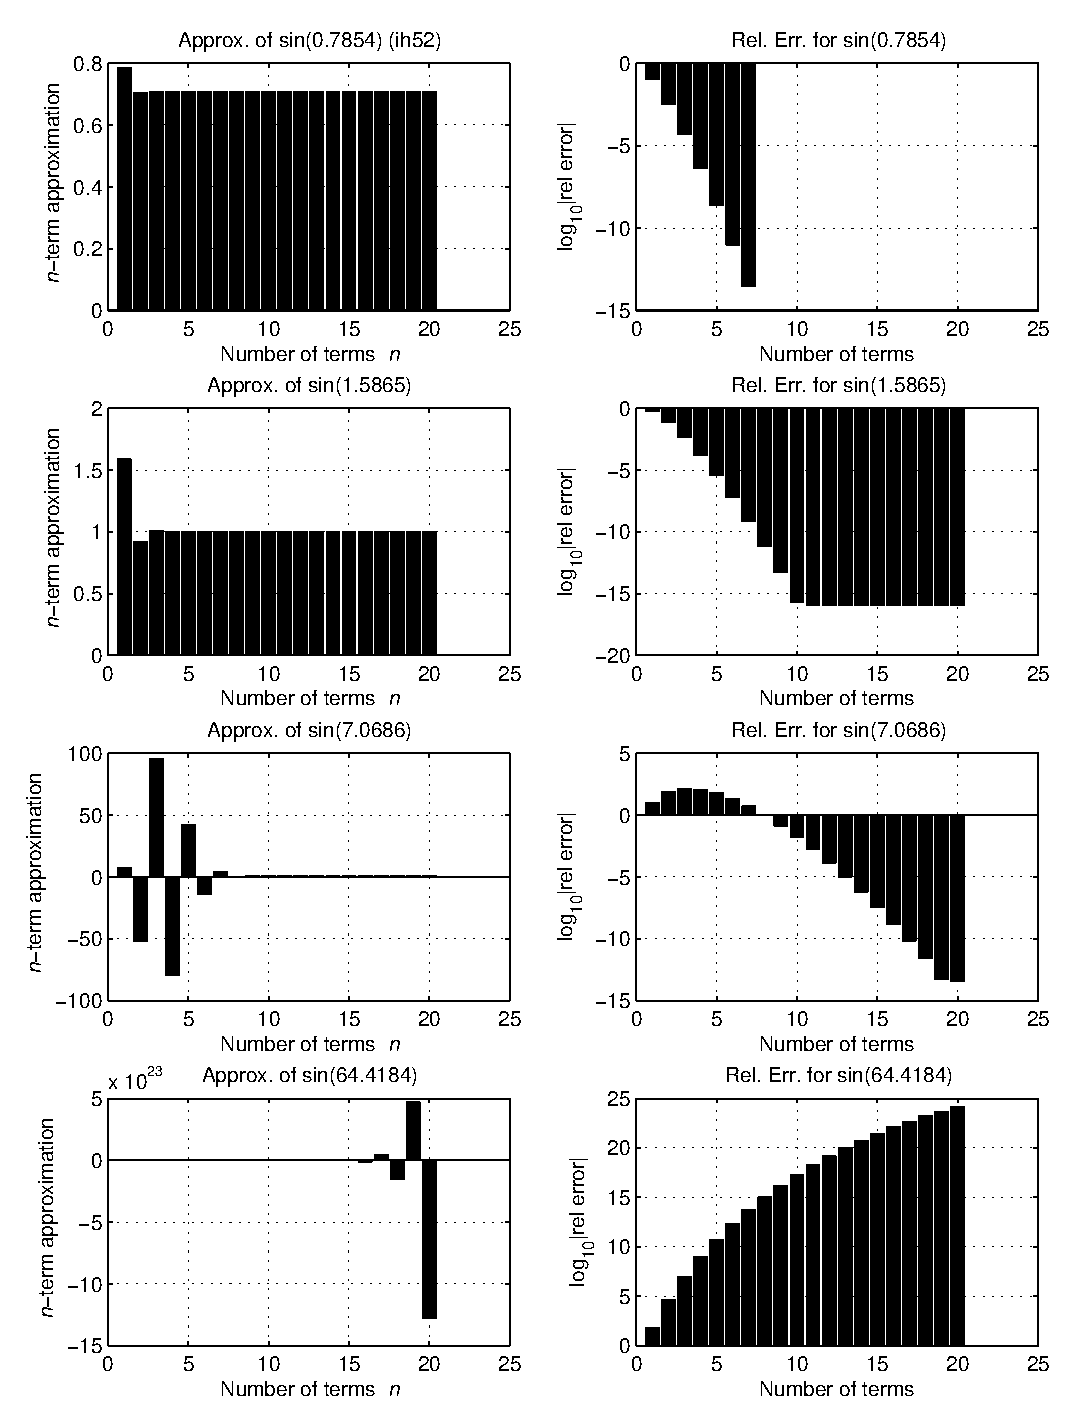
\epsfig{file=SinSeriesCheckerPlot.eps, width=6in}
\caption{Output of {\tt SinSeriesChecker.m} for Chapra 3.5}
\end{center}
\end{figure}

% As for the rest, 4.5in is usually fine
% Don't forget to remove % in front of \epsfig!
\begin{figure}[ht!]
\begin{center}
%\epsfig{file=SAMPLE.eps, width=4.5in}
\caption{CAPTION.}
\end{center}
\end{figure}

\clearpage % start bibliography on new page

\begin{thebibliography}{9}
\bibitem{Chapra}
  Chapra, Steven C.,
  {\it Applied Numerical Methods with MATLAB for Engineering and Scientists}.
  McGraw-Hill, New York,
  3rd Edition,
  2012.
\bibitem{Palm}
  Palm, William J.,
  {\it Introduction to MATLAB for Engineers}.
  McGraw-Hill, New York,
  3rd Edition,
  2011.
\bibitem{Other}
  Other source here...  Probably Wikipedia.
\end{thebibliography}

\end{document}
